\section{Drell-Yan Cross Section in QCD}\label{sec:Drell-Yan Hadronic Cross Section}
In this section we will make another calculation that historically has been important in the study of QCD, namely the Drell-Yan process.  

In 1970, the first observation of a $\mu^{+}\mu^{-}$ in hadron-hadron collision was observed \cite{Christenson:1970um}. By applying the parton model Drell and Yan were the first to give a theoretical prediction of this process \cite{Drell:1970wh}. In the modern framework of QCD, the impulse approximation of the parton model is as in DIS replaced by the more precise concept of factorization. Then it can be proven that the hadronic Drell-Yan cross section can be written as a convolution of a perturbative calculable partonic cross section and universal process independent parton distribution functions \cite{Collins:1989gx}. Without specifying the kinematics, the hadronic cross section can be written as
\begin{align}
  \sigma_{h_1\,h_2}(P_1,P_2)=\sum_{i,j}\int dx_1\,dx_2\,f_{i/h_1}(x_1,\mu_{F})f_{j/h_1}(x_1,\mu_{F})\,\hat{\sigma}_{ij}(x_1P_1,x_2P_2,\mu_{F})\,,
\end{align}
which is the form we expected from the parton model, and as in DIS, the parton distribution functions and the partonic cross section has acquired an dependancy on the factorization scale. 

In the simplest case, a Drell-Yan process is the annihilation of a quark-antiquark pair into a virtual photon, which subsequently produces a pair of leptons with invariant mass $Q^{2}$. As leptons are blind to the strong interaction, there will not be any final state gluon radiation. The consequence is that all radiation comes from the initial state quark-antiquark pair, and therefore we have a clear probe of the behaviour of coloured particles. Consequently, the Drell-Yan process is an effective way of studying the internal structure of hadrons.

The main objective of this section is to investigate the divergences appearing in higher-order calculations, and how to deal with them using renormalization techniques. The calculation will proceed through the use of dimensional regularization, where the poles will manifest themselves in $1/\epsilon$. Further, close to the threshold, the finite result has contributions that become large, and these must eventually be handled using resummation techniques. To this end, we will focus on the next-to-leading order (NLO) calculation, where the initial state quarks emit a gluon.

\subsection{LO Drell-Yan Cross Section}
For the sake of completeness we will first sketch the leading order result. At this order we write the partonic process as $q(p)+\bar{q}(p')\rightarrow l^{-}(k)+l^{+}(k')$, where the corresponding Feynman diagram is given in \cref{fig:Drell-Yan LO}.
\begin{figure}
  \centering
  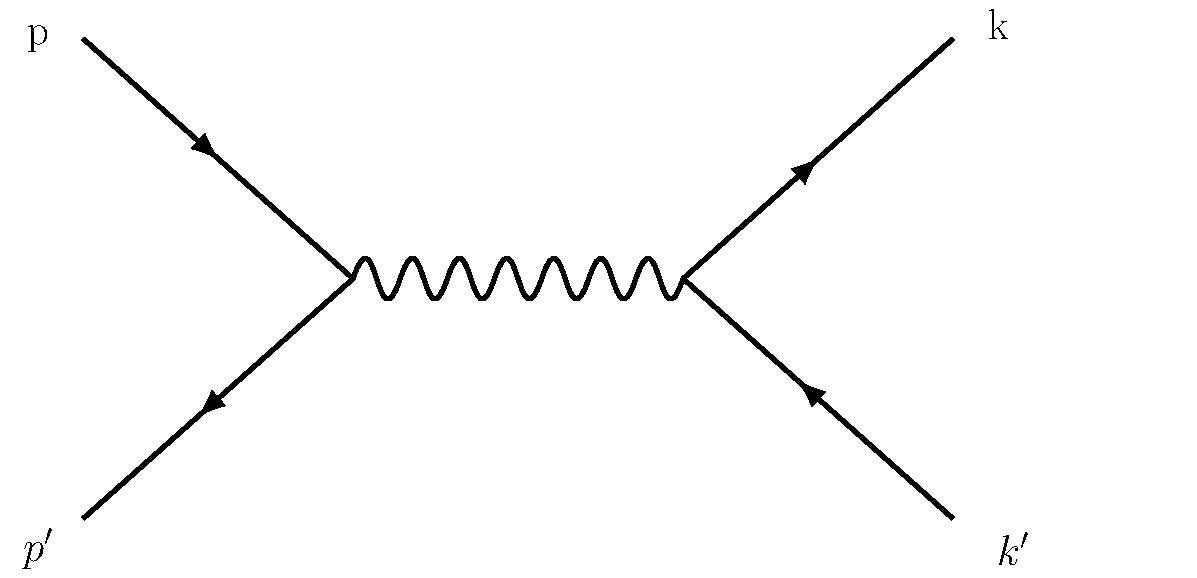
\includegraphics[scale=0.4]{Figures/DrellYanLO}
  \caption{Drell-Yan process at leading order.}
  \label{fig:Drell-Yan LO}
\end{figure}\noindent
Here $p$ and $p'$ denote the momenta of the incoming quark and antiquark, and likewise $k$ and $k'$ denote the momentum of the outgoing leptons. We can directly write down the amplitude from the basic Feynman rules\footnote{To see where all these term comes from, see \cref{eq:QED feynman rule} for the quark-photon vertex, \cref{eq:photon propagator without gauge choice} for the photon propagator and \cref{sec:canonical quantization free theories} for the appearance of spinors.}
\begin{align}
    i\mathcal{M}=i\delta_{ij}\frac{Q_{q}e^{2}}{q^{2}}\big[\bar{v}(p')\gamma^{\mu}u(p)\big]\big[\bar{u}(k)\gamma_{\mu}v(k')\big]\,,
\end{align}
where $\delta_{ij}$ is a colour conserving factor for the quark vertex, and $Q_{q}$ is the fractional charge of the quarks. As usual we are only interested in the spin and colour averaged amplitude,
\begin{align}
    \langle\,|\mathcal{M}|^{2}\rangle=\frac{1}{N_{c}N_{s}^{2}}\frac{Q_{q}^{2}e^{4}}{\hat{s}^{2}}H^{\mu\nu}L_{\mu\nu}\,,
\end{align}
where $N_c$ and $N_s$ denote the number of colours and spin, and we  have defined hadronic and leptonic tensors
\begin{align}
    H^{\mu\nu}&=\text{Tr}\big[\slashed{p'}\gamma^{\mu}\slashed{p}\gamma^{\nu}\big]\,,
    \\
    L_{\mu\nu}&=\text{Tr}\big[\slashed{k}\gamma_{\mu}\slashed{k'}\gamma_{\nu}\big]\,,
\end{align}
and the contraction yields
\begin{align}
    H^{\mu\nu}L_{\mu\nu}=\hat{s}^{2}(1+\cos\theta^{2})\,,
\end{align}
where $\theta$ is the centre of mass scattering angle, and $\hat{s}$ is the partonic centre of mass energy, $\hat{s}=(p+p')^{2}$. The differential cross section is given by
\begin{align}
    d\hat{\sigma}_{q\bar{q}}^{(0)}=\frac{1}{2\hat{s}}\langle\,|\mathcal{M}|^{2}\rangle d\mathcal{P}^{(2)}\,,
\end{align}
where $d\mathcal{P}^{(2)}$ is the two-body phase space of the final state leptons, see \cref{eq:n-body phase space}. The integrated cross section is given by
\begin{align}
    \hat{\sigma}^{(0)}=\frac{4\pi Q_{q}^{2}\alpha^{2}}{3N_{c}\hat{s}}\,.
\end{align}
We can write this as a differential cross section by using that
\begin{align}
    1=\int dQ^{2}\delta(\hat{s}-Q^{2})\,,
\end{align}
which is merely a statement that the invariant mass of the $q\bar{q}$ pair that annihilates into the photon, matches the invariant mass of the photon. This identity can also be written on the form
\begin{align}
    1=\frac{1}{\hat{s}}\int dQ^{2}\delta(1-\frac{Q^{2}}{\hat{s}})\,,
\end{align}
giving the differential cross section in $Q^{2}$
\begin{align}
    \frac{d\hat{\sigma}_{q\bar{q}}^{(0)}}{dQ^{2}}=\frac{4\pi Q_{q}^{2}\alpha^{2}}{3N_{c}\hat{s}\,Q^{2}}\delta(1-z)=\hat{\sigma}_{0}\,\delta(1-z)\,,
\end{align}
where we defined the partonic Born cross-section $\hat{\sigma}_0=(4\pi Q_{q}^{2}\alpha^{2})/(3N_{c}\hat{s}Q^{2})$, and the partonic threshold variable $z=Q^{2}/\hat{s}$. For later purposes, we want to make some remarks about the structure of the leading order diagram. The photon and leptons do not feel the strong interaction, which means that even at higher orders, the final state part of the amplitude decouples from the initial part. Further, the electromagnetic corrections are negligible compared to the strong corrections so any photon radiation is neglected. To find the higher-order corrections, we only have to consider the corrections for the production of a virtual photon. The leptonic part of the hard process contributes with a factor $\alpha/3Q
^{2}$, where $Q^{2}$ is the invariant mass of the final state leptons.

\begin{figure}
    \centering
    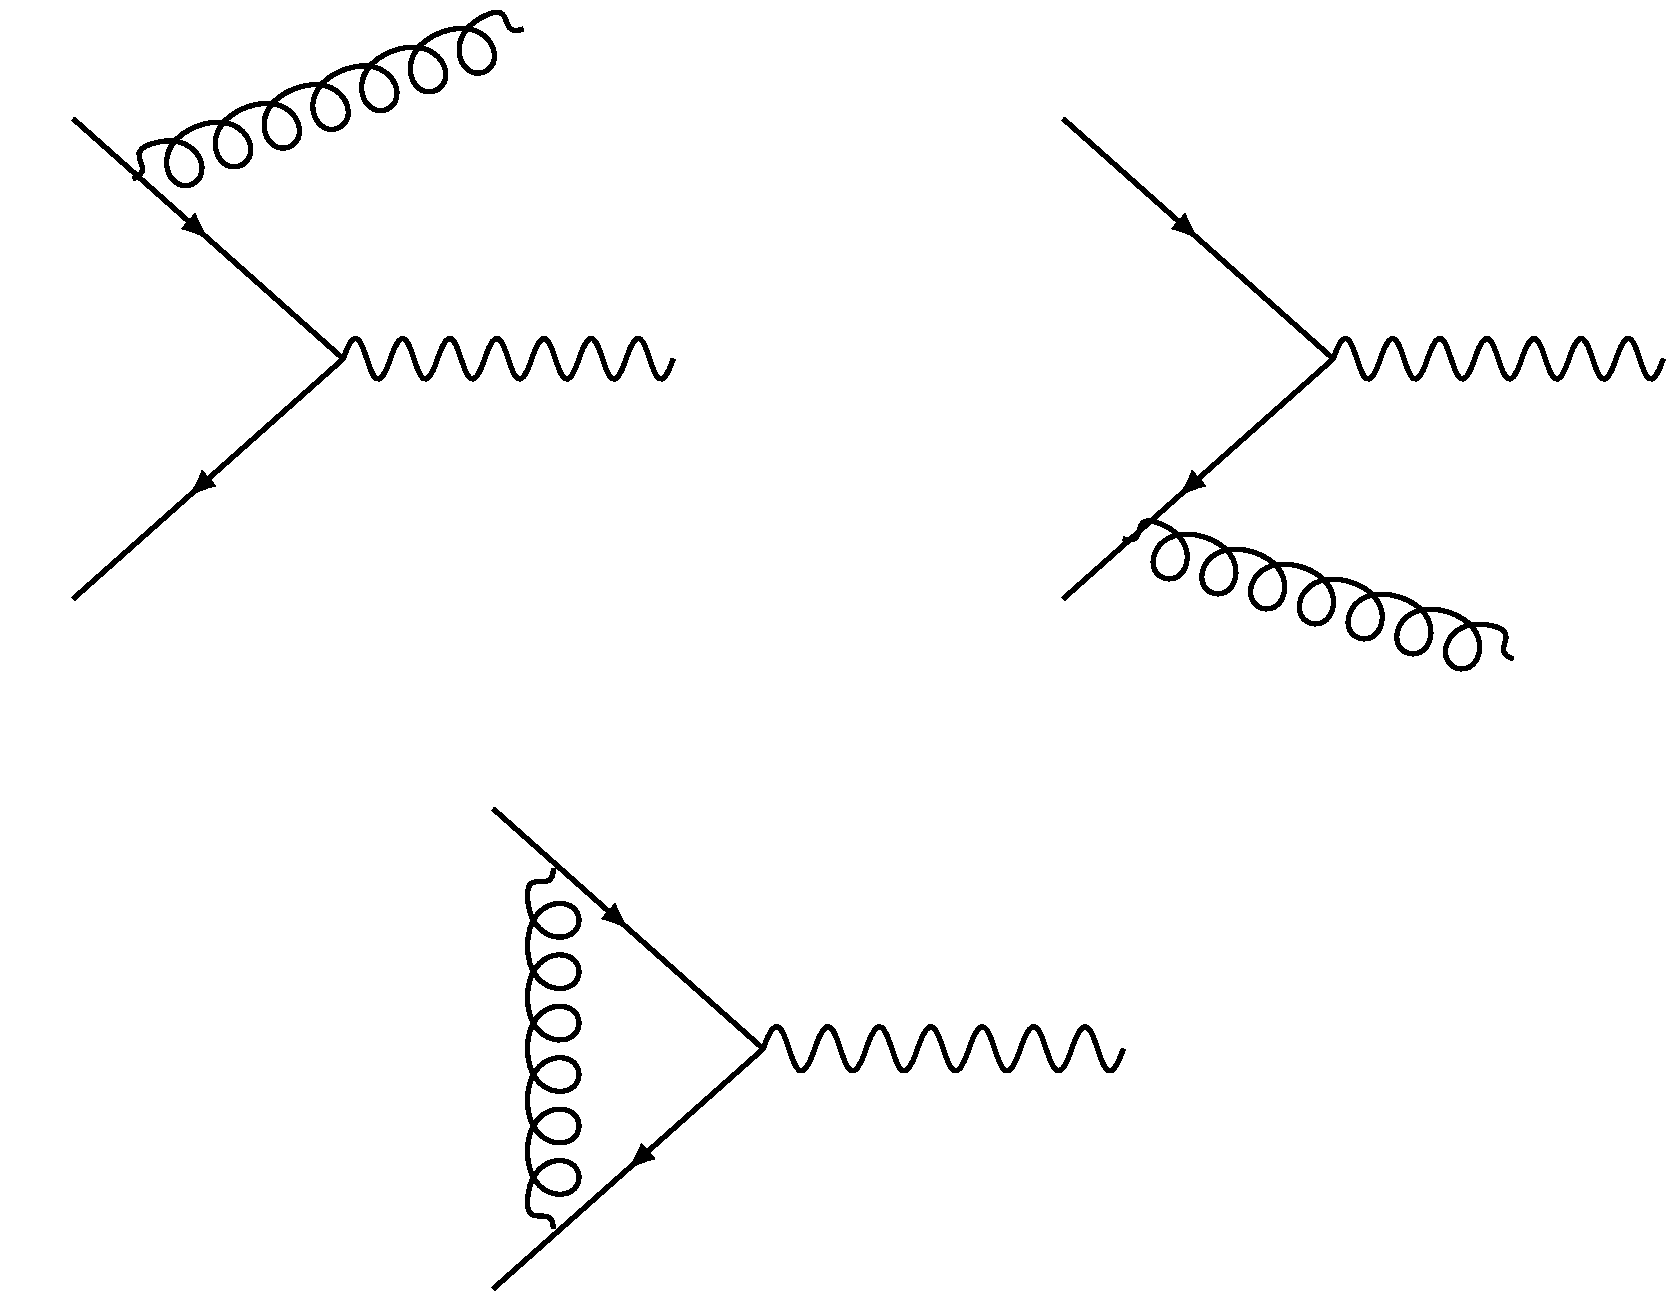
\includegraphics[scale=0.3]{Figures/radiativecorrDY.pdf}
    \caption{NLO diagrams contributing to the Drell-Yan process. Top: Real gluon emission. Bottom: Virtual correction.}
    \label{fig:NLO drell-yan}
\end{figure}
%%%%%%%%%%%%%%%%%%%%%%%%%%%%%%%%%%%%%%%%%%%%%%%%%%%%%%%%%%%%%%%%%%
\subsection{NLO Drell-Yan Cross Section}\label{sec:NLO drell yan calculation}
Let us now go beyond the leading order approximation and calculate the $\mathcal{O}(\alpha_s)$ correction to the Drell-Yan process. The contributing diagrams is illustrated in \cref{fig:NLO drell-yan}, where the upper diagrams corresponds to real gluon emission, and the lower diagram is the virtual correction. As we will see, the difficulty due to divergences in the integral is substantial. To treat these divergences we will use dimensional regularization, see \cref{sec:dimensional regularization} for more detail. One important feature to keep in mind is that the UV-divergences is treated by evaluating $\epsilon>0$ and the IR-divergences for $\epsilon<0$. 

Now, by counting order in $g_s$ in \cref{fig:NLO drell-yan}, we see that the virtual correction has one order higher than the real emission and can not be squared in order to contribute to NLO. Therefore, one must multiply the virtual correction amplitude with the leading order amplitude found from \cref{fig:Drell-Yan LO}, which contributes to wanted order in $\alpha_s$.
The real contribution corresponds to the emission of gluons that are on mass-shell, i.e. there are no undetermined loop momenta that has to be integrated over. However, the phase space integration contains two kinds of singularities. The first is when the gluon is emitted collinearly to the emitting quark. The second singularity appears if the gluon momentum is soft, $k\rightarrow 0$. Both of these divergences are what is called infrared-singularities. Virtual corrections emerge when the initial quarks exchange a gluon. This gluon is virtual, and the integral is over undetermined loop momenta, leading to ultraviolet-divergences. To handle these divergences, we will use dimensional regularization, and work in $d=4-2\epsilon$ dimensions.

\subsection*{Differential cross section}
By applying the QCD Feynman rules, the amplitude for real gluon emission can be written as
\begin{align}
    i\mathcal{M}=&Q_{q}\,e\,g_{s}\,\mu^{(4-d)/2}\,(t^{a}_{ij})\varepsilon_{\alpha}^{*}(k)\varepsilon_{\mu}^{*}(q)\big[\bar{v}(p')A^{\mu\alpha}u(p)\big]\,,
\end{align}
where we have made the usual substitution $g_{s}\rightarrow \mu^{\epsilon}g_s$. We have also used the abbreviation
\begin{align}
    A^{\mu\alpha}=\gamma^{\mu}\frac{i(\slashed{p}-\slashed{k})}{(p-k)^{2}}\gamma^{\alpha}+\gamma^{\alpha}\frac{i(\slashed{p}-\slashed{q})}{(p-q)^{2}}\gamma^{\mu}\,,
\end{align}
where $k$ is the gluon momenta and $q$ is the massive photon momenta. The spin and colour averaged amplitude is given by
\begin{align}\label{eq:ugly NLO averaged amplitude DY}
    \langle\,|\mathcal{M}|^{2}\rangle&=\mathcal{C}\frac{Q_{q}^{2}e^{2}g_{s}^{2}\mu^{(4-d)}}{N_{s}^{2}}\text{Tr}[\slashed{p'}A^{\mu\alpha}\slashed{p}A_{\alpha\mu}]\nonumber
    \\
    &=C_{F}\frac{Q_{q}^{2}e^{2}g_{s}^{2}\mu^{(4-d)}}{N_{c}\,N_{s}^{2}}\,2(d-2)\Big(2\hat{s}\frac{Q^{2}}{\hat{t}\hat{u}}+2(d-4)+(d-2)\Big[\frac{\hat{t}}{\hat{u}}+\frac{\hat{u}}{\hat{t}}\Big]\Big)\nonumber
    \\
    &=C_{F}\frac{Q_{q}^{2}e^{2}g_{s}^{2}\mu^{2\epsilon}}{N_{c}\,N_{s}^{2}}\,8(1-\epsilon)\Big(2\hat{s}\frac{Q^{2}}{\hat{t}\hat{u}}-2\epsilon+(1-\epsilon)\Big[\frac{\hat{t}}{\hat{u}}+\frac{\hat{u}}{\hat{t}}\Big]\Big)\,,
\end{align}
where the terms with $d=4-2\epsilon$ appears because of the modified Dirac algebra in $d$-dimensions \cref{sec:Appendix Dirac gamma matrices}. The color factor for this process follows from the QCD group structure\footnote{See \cite{Peskin:257493} for a more elaborate treatment of the colour sums.} 
\begin{align}
    \mathcal{C}=\frac{1}{N_{c}}\text{Tr}[t^{a}t^{a}]=\frac{C_{F}}{N_C}\,,
\end{align}
and the partonic Mandelstam variables is defined as
\begin{align}\label{eq:partonic Mandelstam}
    \hat{s}&=(p+p')^{2}=(q+k)^{2}\,,
    \\
    \hat{t}&=(p-q){2}=(p'-k)^{2}\,,
    \\
    \hat{u}&=(p-k)^{2}=(p'-q)^{2}\,.
\end{align}
The partonic differential cross section is then given by
\begin{align}
    \frac{d\hat{\sigma}_{q\bar{q}}^{r}}{dQ^{2}}=\frac{1}{2}\Big(\frac{\alpha}{3Q^{2}}\Big)\int\,d\mathcal{P}^{(2)}\,\langle\,|\mathcal{M}|^{2}\rangle\,,
\end{align}
where the bracket represents lepton part appearing at all order. The differential phase space is over the massless gluon momenta $k$ and the virtual photon momenta $q$. In $d$-dimensions, the differential phase space can be written as
\begin{align}
    d\mathcal{P}=\frac{1}{8\pi}\Big(\frac{4\pi}{Q^{2}}\Big)^{\epsilon}\frac{(1-z)^{1-2\epsilon}\,z^{\epsilon}}{\Gamma(1-\epsilon)}\big(y(1-y))\big)^{-\epsilon}\,dy\,,
\end{align}
where $y=\frac{1}{2}(1+\cos\theta)$, $\Gamma$ is the Euler-Gamma function and z is the threshold variable $z=Q^{2}/\hat{s}$. Notice that the integral is to be taken over the dimensionless quantity $y$, so we should find a way of rewriting the averaged amplitude in terms $y$ as well. We already have the partonic centre of mass-energy, $\hat{s}$ in terms of $z$, so by writing out $\hat{t}$ and $\hat{u}$ we find
\begin{align}
    \hat{t}&=-\frac{Q^{2}}{z}(1-z)(1-y)\,,
    \\
    \hat{u}&=-\frac{Q^{2}}{z}(1-z)y\,.
\end{align}
With these definitions, the averaged amplitude in \cref{eq:ugly NLO averaged amplitude DY} takes the form
\begin{align}
     \langle\,|\mathcal{M}|^{2}\rangle&=C_{F}\frac{Q_{q}^{2}e^{2}g_{s}^{2}\mu^{2\epsilon}}{N_{c}\,N_{s}^{2}}\,8(1-\epsilon)\Big(\frac{2z}{(1-z)^{2}(1-y)y}\nonumber
     \\
     &\hspace{0.2cm}+(1-\epsilon)\Big[\frac{1-y}{y}+\frac{y}{1-y}\Big]-2\epsilon\Big)\,.
\end{align}
At this point it is worth commenting the different terms in this expression: we have that $(1-z)$ is the momentum fraction of the emitted gluon, and if the gluon is soft, $z=1$, we have a singularity. Further, if the gluon is emitted collinearly to the emitting quarks, we have that $y=1$, resulting in another singularity. Hence, we have both a collinear and soft divergence.

However, if we keep $\epsilon$ finite, the singularities can be extracted by using the Euler-Beta integral. The singularities will then manifest themselves in $\epsilon$ singularities. Writing out all terms, the differential cross-section for real emission takes the form
\begin{align}
    \frac{d\hat{\sigma}_{q\bar{q}}^{r}}{dQ^{2}}&=\frac{1}{2\hat{s}}\Big(\frac{\alpha}{3\pi Q^{2}}\Big)\Big[C_{F}\frac{Q_{q}^{2}e^{2}g_{s}^{2}\mu^{2\epsilon}}{N_{c}\,N_{s}^{2}}\Big]\frac{1}{8\pi}\Big(\frac{4\pi}{Q^{2}}\Big)^{\epsilon}\frac{(1-z)^{1-2\epsilon}\,z^{\epsilon}}{\Gamma(1-\epsilon)}8(1-\epsilon)\nonumber
    \\
    &\hspace{0.3cm}\times\int_{0}^{1}dy\,\big(y(1-y)\big)^{-\epsilon}\Big(\frac{2z}{(1-z)^{2}(1-y)y}+(1-\epsilon)\Big[\frac{1-y}{y}+\frac{y}{1-y}\Big]-2\epsilon\Big)\nonumber
    \\
    &=C_{F}\hat{\sigma}_{0}\frac{\alpha_s}{2\pi}\Big(\frac{4\pi\mu^{2}}{Q^{2}}\Big)^{\epsilon}\frac{(1-\epsilon)}{\Gamma(1-\epsilon)}(1-z)^{1-2\epsilon}z^{\epsilon}\nonumber
    \\
    &\hspace{0.3cm}\times\Big[\frac{2z}{(1-z)^{2}}B(-\epsilon,-\epsilon)+2(1-\epsilon)B(-\epsilon,2-\epsilon)-2\epsilon B(1-\epsilon,1-\epsilon)\Big]\nonumber
    \\
    &=C_{F}\hat{\sigma}_{0}\frac{\alpha_s}{\pi}A(\epsilon)\frac{z^{\epsilon}}{\epsilon}\Big(-2z(1-z)^{-1-2\epsilon}-(1-z)^{1-2\epsilon}\Big)\,,
\end{align}
where we for notational simplicity have neglected several factors that are finite for $\epsilon\rightarrow 0$. The integral over $y$ was performed by the Euler-Beta integral
\begin{align}
    B(a,b)=\int_{0}^{1}dt\,t^{a-1}(1-t)^{b-1}=\frac{\Gamma(a)\Gamma(b)}{\Gamma(a+b)}\,,
\end{align}
and we defined the prefactor $A(\epsilon)$ as
\begin{align}
    A(\epsilon)=\Big(\frac{4\pi\mu^{2}}{Q^{2}}\Big)^{\epsilon}\frac{\Gamma(1-\epsilon)}{\Gamma(1-2\epsilon)}\,.
\end{align}

We still have a singularity as $z\rightarrow 1$. To make all singularities manifest in $\epsilon$, we can expand the terms inside the bracket by the use of plus distributions, see \cref{sec:Appendix Plus Distributions}. We write this as
\begin{align}\label{eq:DRell Yan plus distribution example}
    (1-z)^{-1-2\epsilon}&=-\frac{1}{2\epsilon}\delta(1-z)+\Big[\frac{1}{1-z}\Big]_{+}-2\epsilon\Big[\frac{\ln(1-z)}{1-z}\Big]_{+}+\mathcal{O}(\epsilon^{2})\,,
    \\
    z^{\epsilon}&=1+\epsilon \ln z+\mathcal{O}(\epsilon^{2})\,.
\end{align}
With these considerations, the final result for real gluon emission takes the form
\begin{align}
    \frac{d\hat{\sigma}_{q\bar{q}}^{r}}{dQ^{2}}=C_{F}&\hat{\sigma}_{0}\frac{\alpha_s}{\pi}A(\epsilon)\Big(\frac{1}{\epsilon^{2}}\delta(1-z)-\frac{1}{\epsilon}\Big[\frac{1+z^{2}}{1-z}\Big]_{+}\,,\nonumber
    \\
    &+2(1+z^{2})\Big[\frac{\ln(1-z)}{(1-z)}\Big]_{+}-\frac{1+z^{2}}{1-z}\ln z\Big)\,.
\end{align}

We have now managed to bring all singularities on $\epsilon$ form. The term $1/\epsilon^{2}$ is an infrared singularity due to simultaneously soft and collinear emission, and the term $1/\epsilon$ is due to collinear emission. 

To any given order in perturbation theory, we must consider all possible diagrams at that specific order and add them at the end. Therefore, we must find the virtual contribution and see if some of the singular terms cancel. The only virtual contribution comes from the lower diagram in \cref{fig:NLO drell-yan}. There are two additional diagrams at this order that could contribute, the quark self-energy diagrams, but it can be shown that these exactly cancel each other. The virtual contribution contains both infrared and ultraviolet-singularities. To separate these singularities, we do as in \cref{eq:scaleless integral} and name them $\epsilon_{UV}$ and $\epsilon_{IR}$. 

The amplitude for the virtual correction is given by
\begin{align}\label{eq:DY virtual amplitude}
    \mathcal{M}^{\mu}=&t_{ik}^{a}t_{kj}^{a}\mu^{(4-d)}\int\frac{d^{d}k}{(2\pi)^{2}}\bar{v}(p')(ig_s\gamma^{\alpha})\frac{i(\slashed{p'}+\slashed{k})(ie\gamma^{\mu})i(\slashed{k}-\slashed{p}))}{(p'+k)^{2}(p-k)^{2}}(ig_s\gamma^{\beta})u(p)\,D_{\alpha\beta}(k)\nonumber
    \\
    &=eg_s^{2}C_{F}\mu^{(d-4)}\int\frac{d^{d}k}{(2\pi)^{2}}\bar{v}(p')\gamma^{\alpha}\frac{(\slashed{p'}+\slashed{k})\gamma^{\mu}(\slashed{k}-\slashed{p})}{k^{2}(p'+k)^{2}(p-k)^{2}}\gamma^{\beta}u(p)\nonumber
    \\
    &=\bar{v}(p')(\Gamma^{\mu})u(p)\,,
\end{align}
where we have defined the vertex correction $\Gamma^{\mu}$. The integrand can be simplified by the Dirac algebra in $d$-dimensions and the massless Dirac equation. Further, by applying the Feynman parameter method introduced in \cref{sec:dimensional regularization}, the integral can be turned into a Euler-Beta integral. 

The propagator factors in \cref{eq:DY virtual amplitude}, are the same as the ones we derived in \cref{eq:virtual gluon feynman parametrization}. The numerator is straightforward to manipulate, but tedious. The resulting vertex correction is given by
\begin{align}
    \Gamma^{\mu}=\gamma^{\mu}&C_{F}\frac{\alpha_s}{4\pi}\Big(\frac{4\pi\mu^{2}}{Q^{2}}\Big)^{\epsilon}(-1)^{\epsilon}\Gamma(1+\epsilon)\Gamma(1-\epsilon)\frac{\Gamma(1-\epsilon)}{\Gamma(1-2\epsilon)}\nonumber
    \\
    &\Big(\frac{1}{\epsilon_{UV}}-\frac{2}{\epsilon_{IR}^{2}}-\frac{4}{\epsilon_{IR}}-8+\mathcal{O}(\epsilon)\Big)\nonumber
    \\
    &=\gamma^{\mu}C_{F}\frac{\alpha_s}{4\pi}A(\epsilon)\Big(\frac{1}{\epsilon_{UV}}-\frac{2}{\epsilon_{IR}^{2}}-\frac{4}{\epsilon_{IR}}-8+\frac{2\pi^{2}}{3}+\mathcal{O}(\epsilon)\Big)\,,
\end{align}
where we expanded the factors
\begin{align}
    (-1)^{\epsilon}\Gamma(1+\epsilon)\Gamma(1-\epsilon)=1-\frac{\pi^{2}}{3}\epsilon^{2}+\mathcal{O}(\epsilon^{3})\,.
\end{align}
To regulate the UV-singularities we have to add a counterterm. We are not considering electroweak corrections, so for our vertex correction the only reasonable counterterm to add is the quark self-energy. In dimensional regularization this contribution yields a scaleless integral, which we encountered in \cref{eq:scaleless integral}. To remove the UV-divergence we add\footnote{As discussed in \cref{sec:renormalized perturbation theory}, this is always allowed for a renormalizable theory.}
\begin{align}
    \delta_{\Gamma}\gamma^{\mu}=-\gamma^{\mu}C_{F}\frac{\alpha_s}{4\pi}A(\epsilon)\Bigg(\frac{1}{\epsilon_{UV}}-\frac{1}{\epsilon_{IR}}\Bigg)\,.
\end{align}
This results in the UV-finite vertex correction
\begin{align}\label{eq:UV-finite vertex}
    \Gamma_{R}^{\mu}&=\gamma^{\mu}C_{F}\frac{\alpha_s}{4\pi}A(\epsilon)\Big(-\frac{2}{\epsilon_{IR}^{2}}-\frac{3}{\epsilon_{IR}}-8+\frac{2\pi^{2}}{3}+\mathcal{O}(\epsilon)\Big)\nonumber
    \\
    &=\gamma^{\mu}\mathcal{F}\,.
\end{align}

The differential cross section for the virtual correction is obtained by considering the interference between the leading order \cref{fig:Drell-Yan LO} and the vertex correction \cref{fig:NLO drell-yan}. This corresponds to making the substitution 
\begin{align}
    e\gamma^{\mu}\rightarrow\Gamma^{\mu}_{R}=e\gamma^{\mu}\mathcal{F}
\end{align}
which leads to the differential cross section
\begin{align}
    \frac{d\hat{\sigma}_{q\bar{q}}^{v}}{dQ^{2}}&=\frac{d\hat{\sigma}_{q\bar{q}}^{(0)}}{dQ^{2}}2\text{Re}(\mathcal{F})
    \\
    &=C_{F}\hat{\sigma}_{0}\frac{\alpha_s}{\pi}A(\epsilon)\Big(-\frac{1}{\epsilon^{2}}-\frac{3}{2\epsilon}-4+\frac{\pi^{2}}{3}\Big)\delta(1-z)\,.
\end{align}

The real and virtual contributions are now on the same form, such that we can easily add them, giving the NLO result
\begin{align}\label{eq:final NLO partonic qq}
    \Big(\frac{d\hat{\sigma}_{q\bar{q}}}{dQ^{2}}\Big)_{\text{NLO}}&=\frac{d\hat{\sigma}_{q\bar{q}}^{r}}{dQ^{2}}+\frac{d\hat{\sigma}_{q\bar{q}}^{v}}{dQ^{2}}\nonumber
    \\
    &=C_{F}\hat{\sigma}_{0}\frac{\alpha_s}{\pi}A(\epsilon)\Big[-\frac{1}{\epsilon}\Big(\Big[\frac{1+z^{2}}{1-z}\Big]_{+}+\frac{3}{2}\delta(1-z)\Big)+\Big(\frac{\pi^{2}}{3}-4\Big)\delta(1-z)\nonumber
    \\
    &\hspace{1.5cm}+2(1+z^{2})\Big[\frac{\ln(1-z)}{1-z}\Big]_{+}-\frac{1+z^{2}}{(1-z)}\ln z\Big]\,.
\end{align}

We observe that in the sum over real and virtual contributions, some of the divergences have canceled. This is a manifestation of the Kinoshita-Lee-Nauenberg (KLN) theorem \cite{Lee:1964is, Kinoshita:1975bt}. The KLN-theorem states that in the sum of all diagrams, the result is to be free of IR-divergences. But we still have a collinear divergence, which we soon will show how to deal with.  

In general, we can write the partonic cross section as the perturbative expansion
\begin{align}
    \frac{d\hat{\sigma}}{dQ^{2}}&=\sum_{n=0}^{\infty}\Big(\frac{\alpha_s}{\pi}\Big)^{n}\frac{d\hat{\sigma}^{(n)}}{dQ^{2}}\,,\nonumber
    \\
    &=\frac{d\hat{\sigma}^{(0)}}{dQ^{2}}+\frac{\alpha_s}{\pi}\frac{d\hat{\sigma}^{(1)}}{dQ^{2}}+\cdots\nonumber
    \\
    &=\hat{\sigma}_{0}\big(\omega^{(0)}+\frac{\alpha_s}{\pi}\omega^{(1)}+\cdots\big)\,,
\end{align}
where we separated out the Born cross section and defined a hard function $\omega^{(n)}$. With this notation, we have that the hard functions up to $\mathcal{O}(\alpha_s)$ are given by
\begin{align}
    \omega^{(0)}&=\delta(1-z)\,,\nonumber
    \\
    \omega^{(1)}&=-A(\epsilon)\frac{1}{\epsilon}P_{q/q}^{(0)}+A(\epsilon)\Big[\Big(\frac{\pi^{2}}{3}-4\Big)\delta(1-z)\nonumber
    \\
    &\hspace{1.5cm}+2(1+z^{2})\Big[\frac{\ln(1-z)}{1-z}\Big]_{+}-\frac{1+z^{2}}{1-z}\ln z\Big]\,,
\end{align}
where we have inserted the splitting function $P_{q/q}^{(0)}$, see \cref{eq:qq splitting function}.

As mentioned above some of the IR-divergences has canceled, but there still remain a collinear singularity in $1/\epsilon$. The reason this collinear singularity is still present and did not cancel according to the KLN theorem is that we are considering massless particles. To treat the remaining singularity we can use the factorization property of QCD. In DIS we defined \textquote{bare} parton distributions to cancel the divergence. However, we have already seen that we can define parton-in-parton distributions that contains collinear divergences, see \cref{eq:Collins definition of parton-in-parton}. Hence, we can use these parton-in-parton distributions instead, which we will show how to do in the next section.

%recall the underlying assumption behind the factorization theorem in QCD. The hadronic cross section could be factorized in a hard scattering part convoluted with the universal parton distribution functions. The hard part describes the physics on short scale, and the parton distribution functions describes the physics on long scale. The crucial point is that the only observable quantity is the hadronic cross section, meaning that we can renormalize the cross section by refactorizing the partonic cross section using parton-in-parton distributions.

\subsection{Renormalization of NLO cross section}\label{sec:renormalizing drell-yan}
According to the QCD factorization theorem, the hadronic Drell-Yan cross section can be written as\footnote{This is proven to hold up to corrections of $\mathcal{O}(1/Q^{2})$, see \cite{Collins:1989gx}. In \cref{sec:NLO drell yan calculation} we only considered the $q\bar{q}$ process, but to be general we will use generic subscripts.}
\begin{align}\label{eq:Factorized hadronic Dre-Yan}
   \frac{ d\sigma_{h_1h_2}}{dQ^{2}}=\sigma_{0}W(\tau,Q,\mu,\alpha_s)\,,
\end{align}
where\footnote{This is really a Mellin convolution, see \cref{sec:Appendix Mellin Transform}.}
\begin{align}\label{eq:hadronic convolution}
    W(\tau,Q,\mu,\alpha_s)=\sum_{i,j}Q_{q}^{2}\int \frac{dx_{1}}{x_1}\frac{dx_{2}}{x_2}f_{i/h_1}(x_1,\mu)f_{j/h_2}(x_2,\mu)w_{ij}\Big(z,Q,\mu,\alpha_{s}(\mu)\Big)\,,
\end{align}
where we set the factorization and renormalization scale to be the same, $\mu_F=\mu_R=\mu$. We have also factored out the hadronic Born cross section by using that $x_{1}x_{2}\bar{\sigma_{0}}=Q_{q}^{2}\sigma_{0}$, where
\begin{align}
    \sigma_{0}=\frac{4\pi\alpha^{2}}{3N_{c}sQ^{2}}
\end{align}
and defined the hadronic and partonic threshold variables as
\begin{align}
    \tau=\frac{Q^{2}}{s}\,,\hspace{1cm}z=\frac{\tau}{x_{1}x_{2}}\,.
\end{align}

The singular part of the fixed order calculation needs to be separated out of the hard scattering part, such that we can absorb it into the parton distribution functions. To this end, we define the partonic analogue to \cref{eq:hadronic convolution}
\begin{align}\label{eq:refactorized partonic drell-yan}
   h_{ij}(z,Q,\mu,\alpha_{s}(\mu),\epsilon)=&\sum_{k,l}\int_{z}^{1}\frac{dy_{1}}{y_{1}}\frac{dy_{2}}{y_{2}}\,f_{k/i}(y_1,\mu,\epsilon)\,f_{l/j}(y_2,\mu,\epsilon)\nonumber
   \\
   &\times\omega_{ij}\Big(\frac{z}{y_1},\frac{z}{y_2},Q,\mu,\alpha_{s}(\mu^{2})\Big)
\end{align}
which is a refactorization of the hard scattering function using the parton-in-parton densities we discussed in \cref{sec:lightcone parton in parton distributions}. We can extract the singular part by making the following perturbative expansion
\begin{align}\label{eq:perturbative expansion DY refactorization}
  h_{ij}=h_{ij}^{(0)}+\frac{\alpha_s}{\pi}h_{ij}^{(1)}+\mathcal{O}(\alpha_{s}^{2})
  \\
  \omega_{ij}=\omega_{ij}^{(0)}+\frac{\alpha_s}{\pi}w_{ij}^{(1)}+\mathcal{O}(\alpha_{s}^{2})
  \\
  f_{i/j}=f_{i/j}^{(0)}+\frac{\alpha_s}{\pi}f_{i/j}^{(1)}+\mathcal{O}(\alpha_{s}^{2})\,,
\end{align}
where $h_{ij}^{(1)}$ is the singular hard function we calculated at NLO in \cref{sec:NLO drell yan calculation}, i.e.
\begin{align}
  h_{ij}^{(1)}&=-A(\epsilon)\frac{1}{\epsilon}P_{q/q}^{(0)}+A(\epsilon)\Big(\frac{\pi^{2}}{3}-4\Big)\delta(1-z)\nonumber
    \\
    &\hspace{1.5cm}+2(1+z^{2})\Big[\frac{\ln(1-z)}{1-z}\Big]_{+}-\frac{1+z^{2}}{1-z}\ln z\,,
\end{align}
and the $\mathcal{O}(\alpha_s)$ parton-in-parton density is given in \cref{eq:quark in quark PDF to one-loop}. Let us expand $A(\epsilon)$, giving
\begin{align}
    A(\epsilon)=\Big(\frac{4\pi\mu^{2}}{Q^{2}}\Big)^{\epsilon}\frac{\Gamma(1-\epsilon)}{\Gamma(1-2\epsilon)}=1-\epsilon(\gamma_{E}-\ln{4\pi})+\epsilon\ln\Big(\frac{\mu^{2}}{Q^{2}}\Big)+\mathcal{O}(\epsilon^{2})\,.
\end{align}
By using the $\overline{\text{MS}}$ scheme we remove $\gamma_E$ and $\ln(4\pi)$, giving
\begin{align}
    h_{ij}^{(1)}(z,\epsilon)&=C_F\Big[\Big(\frac{\pi^{2}}{3}-4\Big)\delta(1-z)+2(1+z^{2})\Big[\frac{\ln(1-z)}{1-z}\Big]_{+}-\frac{1+z^{2}}{1-z}\ln z\Big]\nonumber
    \\
    &\hspace{0.5cm}-\frac{1}{\epsilon}\Big(1+\epsilon\ln{\frac{\mu^{2}}{Q^{2}}}\Big)P_{q/q}^{(0)}(z)\,,
    \\
    f_{i/j}^{(1)}(z,\epsilon)&=-\frac{1}{2\epsilon}\Big[1+\epsilon\ln\big(\frac{\mu^{2}}{\mu_{F}^{2}}\big)\Big]P_{q/q}^{(0)}(z)\,.
\end{align}
If we insert the perturbative expansions in \cref{eq:perturbative expansion DY refactorization} into \cref{eq:refactorized partonic drell-yan}, we find that
\begin{align}
    h_{ij}^{(0)}(z)=\omega_{ij}^{(0)}(z)=\delta_{ij}\delta(1-z)\,,
\end{align}
and the first order correction is given by
\begin{align}
  \omega_{ij}^{(1)}(z)&=h_{ij}^{(1)}(z,\epsilon)+\frac{1}{2\epsilon}\Big[1+\epsilon\ln\Big(\frac{\mu^{2}}{\mu_{F}^{2}}\Big)\Big]\sum_{k}\int_{z}^{1}\frac{dy_1}{y_1}P_{k/i}^{(0)}(y_1)h_{kj}^{(0)}(\frac{z}{y_1})\nonumber
  \\
  &\hspace{1cm}+\frac{1}{2\epsilon}\Big[1+\epsilon\ln\Big(\frac{\mu^{2}}{\mu_{F}^{2}}\Big)\Big]\sum_{l}\int_{z}^{1}\frac{dy_2}{y_1}P_{l/j}^{(0)}(y_2)h_{il}^{(0)}(\frac{z}{y_2})\nonumber
  \\
  &=h_{ij}^{(1)}(z,\epsilon)+\frac{1}{\epsilon}P_{ij}^{(0)}(z)+\ln\Big(\frac{\mu^{2}}{\mu_{F}^{2}}\Big)P_{ij}^{(0)}(z)\nonumber\,,
\end{align}
where we used the delta function to evaluate the integrals.
We observe that the $1/\epsilon$ singularity will cancel in this sum, leading to the infrared safe hard function in the $\overline{MS}$-scheme
\begin{align}\label{eq:infrared safe hard function}
    \omega_{q\bar{q}}^{(1)}(z)&=P_{qq}^{(0)}\ln{\frac{Q^{2}}{\mu_{F}^{2}}}+C_{F}\Big[\Big(\frac{\pi^{2}}{3}-4\Big)\delta(1-z)\nonumber
    \\
    &\hspace{0.3cm}+2(1+z^{2})\Big[\frac{\ln(1-z)}{1-z}\Big]_{+}-\frac{1+z^{2}}{1-z}\ln z\Big]\,.
\end{align}
Hence, regularizing soft divergences gives rise to logarithmic plus distributions and regularizing collinear divergences gives rise to a logarithm of the factorization scale.

We can remove this last part by choosing $\mu_F=Q$, which also removes the splitting function that contains further plus distributions. This is the most common choice in the literature, which we also adopt. With this choice the partonic scattering function up to $\mathcal{O}(\alpha_s)$ takes the form
\begin{align}\label{eq:NLO drell yan hard function}
    \omega_{q\bar{q}}(z,\alpha_{s}(\mu))&=\delta(1-z)+\frac{\alpha_{s}}{\pi}C_{F}\Big[\Big(\frac{\pi^{2}}{3}-4\Big)\delta(1-z)\nonumber
    \\
    &\hspace{0.3cm}+2(1+z^{2})\Big[\frac{\ln(1-z)}{1-z}\Big]_{+}-\frac{1+z^{2}}{1-z}\ln z\Big]\,.
\end{align}

The result in \cref{eq:NLO drell yan hard function} contains no singularities, but the plus distributions is a source of potential large corrections. When we are close to threshold, there is little phase space left for the emission of gluons. In this case, most of the energy is used to produce the final state leptons, leading to a suppression of real soft gluon emission\footnote{These are soft because near threshold most of the energy is used to produce the final state leptons.}. These plus distributions appeared when we summed real and virtual contributions. Thus, if real contributions are suppressed there will be an imbalance in the cancellation. These corrections appear to all order in perturbation theory, so to $n$-th order they take the form
\begin{align}
    \alpha_{s}^{n}\Big[\frac{\ln^{2n-1}(1-z)}{1-z}\Big]_{+}\,.
\end{align}
As they are large in the threshold regime, they will spoil the convergent behaviour of the perturbative expansion. Therefore, they must be treated to all orders in order to make reliable predictions. The technique to do this is called \emph{threshold resummation}, which we will lay out in more detail in the next chapter.


\subsection{Numerical Evaluation of the Hadronic Drell-Yan Cross Section}
In this section we will compare the LO and the full NLO differential cross section for the Drell-Yan process to experimental results from the CMS experiment \cite{Sirunyan:2018owv}. Our basic result is shown in \cref{fig:numerical LO and NLO cross section} where the LO result is given by the dashed line, the full NLO result in the solid line and the data from CMS is given by the red dots with errorbars \cite{Sirunyan:2018owv}. The numerical evaluation is based on the analytical $\mathcal{O}(\alpha_s)$ result in \cref{eq:NLO drell yan hard function} and performed by evaluating \cref{eq:Factorized Dre-Yan Cross Section} for both the LO and LO$+$NLO cross section. The analytical cross section has been obtained at a centre of mass energy $\sqrt{s}=13$ TeV and we consider production of leptons with invariant mass between 50 and 300 GeV. At LO there is only the $q\bar{q}$ channel that contributes, but at NLO we also have a contribution from a gluon initiated process. To be in accordance with our analytical calculation we have chosen to neglect this contribution in the numerical evaluation as well and only focused on the colour singlet process. Also, the plus distribution in \cref{eq:NLO drell yan hard function} have been omitted as they are to be resummed in \cref{chap:Resummation in QCD}. We use the CT10 NLO \cite{Lai:2010vv} PDF set, and we choose the factorization scale and renormalization scale to be equal the invariant mass of the final state leptons, $\mu=Q$. We have also included the $Z$-boson resonance by using an effective coupling as discussed in \cite{Banfi:2011dm}. 

The main theoretical uncertainty in our analysis comes from the dependence of the calculated cross section on the renormalization and factorization scale. This uncertainty is found by varying the scale between $Q/2$ and $2Q$. By calculating the uncertainty in this way the error-band should give a estimate of how higher order effects should affect the cross section. There are also theoretical uncertainties coming from the PDFs, but we have chosen not to take these into account.

We can see from \cref{fig:numerical LO and NLO cross section} that the full NLO calculation we have performed is much closer to the true cross section found by the CMS experiment than the LO result. This is of course not surprising as the true cross section is an all order process and taking into account higher and higher order in the perturbative expansion should give better and better predictions. However, considering the simplifications we have made by neglecting gluon initiated processes and omitting the plus distribution, the result is surprisingly good. Another point to make is that the dependancy on the renormalization scale is shown to decrease when including QCD effects, implying that even higher order corrections are needed in order to reduce this dependancy even further. Also, according to our uncertainty estimation the full NLO result should lie inside the error-band coming from the LO calculation. But we observe that this is far off, especially at the tails. We suspect that this is due to the fact that at LO we have a pure electroweak process, and QCD effects are only manifest at higher orders. 

\begin{figure}[H]
    \centering
    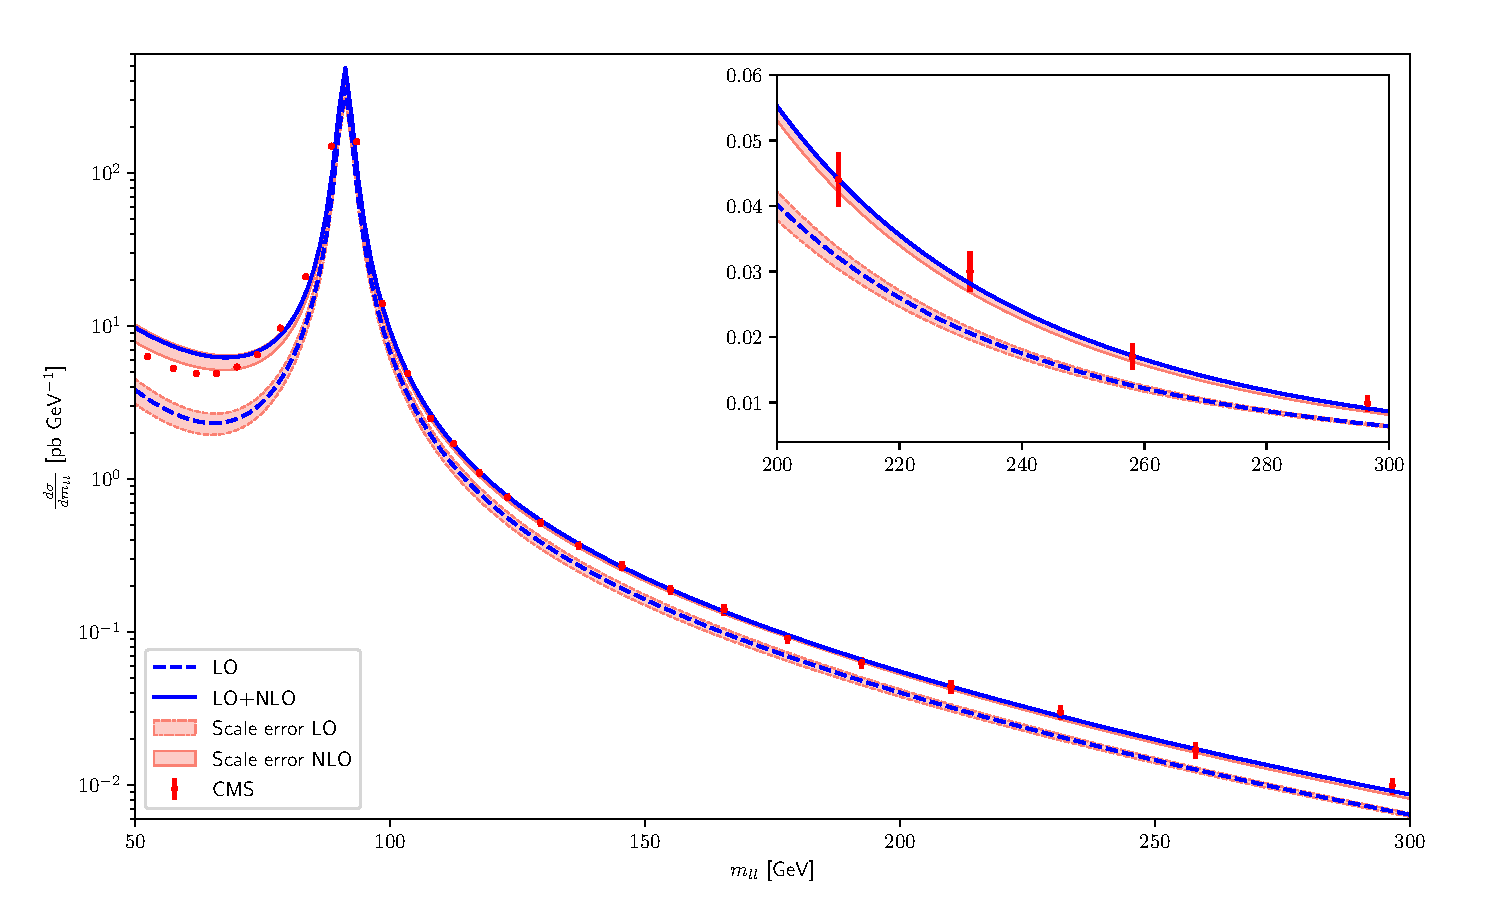
\includegraphics[width=\linewidth]{Figures/dsigmadmll.pdf}
    \caption{Differential cross section of neutral Drell-Yan production as function of final-state invariant mass. Shown are LO (dashed) and LO$+$NLO (solid) results with corresponding scale errors (pink bands). The figure also shows the differential cross section (red dots) measured by the CMS experiment \cite{Sirunyan:2018owv}.}
    \label{fig:numerical LO and NLO cross section}
\end{figure}